% Peekaboo-VL report: 06_results. Included from ../peekaboo_report.tex.
\section{Results}
\label{sec:results}

\subsection{Experimental protocol}
Unless stated otherwise, we report accuracy on our development split
(Sec.~\ref{sec:data}), which mirrors the challenge's ``seen video, new
question'' test regime. Because dev's task mix differs from the test's, we
also report a \emph{test-weighted} accuracy that reweights the eleven tasks
by their test question counts. It predicted the leaderboard within 0.2
points for our first model and within about 1.2 points for the final one,
and it is our model-selection metric. Comparisons between two systems
use a paired exact McNemar test over the questions the two answer
differently. Each configuration is a single run at seed 42: we did not have
the budget for repeated seeds, so our claims rest on paired tests and on
decision rules written down before the run, not on seed averaging. All
models are Qwen3.5-9B in bfloat16 with LoRA adapter weights on the language
model and the vision--language merger (161.6M of 9.57B parameters, 1.69\%);
training runs on one NVIDIA A40 (46\,GB). Decoding is either the official
option order, the four cyclic option permutations averaged (4$\times$ the
cost), or PriDe debiasing~\cite{zheng2024pride} (Sec.~\ref{sec:blind}). We
report failed experiments alongside successful ones. Two systems appear
below: our \emph{first model} (16 frames, 8,000 fit questions), which was
our first leaderboard entry and the reference for most ablations, and the
final \emph{Peekaboo-VL} model (32 frames with random training phases, the
drawn clock on timing questions, all 14,068 fit questions;
Table~\ref{tab:setup}). Recall that 428 dev questions are test questions
(Sec.~\ref{sec:data}).

\subsection{How far do you get without the video?}
Table~\ref{tab:main} shows the main steps, from guessing to our final
system. Without any video, the blind scorer reaches 55.5\% on dev and
55.9\% on the test leaderboard. That is more than double random guessing:
over half of ReVA can be answered without looking at a single frame.
Without any fine-tuning, Qwen3.5-9B already reaches 79.6\% on dev, about the
same as ReMoSense after its full fine-tuning (80.0\% on test).

\begin{table}[t]
\centering
\caption{Overall accuracy (\%). Dev unless marked; ReMoSense numbers are
from its paper (test set).}
\label{tab:main}
\footnotesize
\begin{tabular}{@{}lrr@{}}
\toprule
System & Dev & Test \\
\midrule
Random guessing & 25.0 & 25.2 \\
Longest option / answer-text prior & 41.3 / 40.7 & -- \\
Blind text scorer (ours) & 55.5 & 55.9 \\
\midrule
Qwen3.5-0.8B, no fine-tuning$^\dagger$ & 71.6 & -- \\
\quad + blind prior ($\alpha{=}0.75$ fixed)$^\dagger$ & 77.6 & -- \\
Qwen3.5-4B, no fine-tuning & 77.0 & -- \\
Qwen3.5-9B, no fine-tuning & 79.6 & -- \\
\quad + blind prior ($\alpha$ by cross-validation) & 80.1 & -- \\
\midrule
ReMoSense-7B, fine-tuned~\cite{yao2026reva} & -- & 80.0 \\
First model (16 frames, 8k questions) + PriDe & 84.7 & 82.6 \\
\quad + blind prior ($\alpha$ by cross-validation, not used) & 85.2 & -- \\
\textbf{Peekaboo-VL} (32 frames, clock, all fit), plain & \textbf{85.4} & 83.3 \\
\quad + PriDe letter debiasing (submitted) & 85.0 & \textbf{83.6} \\
\bottomrule
\multicolumn{3}{@{}l@{}}{\scriptsize $^\dagger$On a 250-question dev subset (25 per task, no Viewpoint).}
\end{tabular}
\end{table}


\subsection{Which tasks are still hard?}
Fig.~\ref{fig:pertask} and Table~\ref{tab:pertask} compare the tasks.

The blind scorer does best where the same answers come up again and again:
Viewpoint (72\% on both dev and test) and General Understanding
(71--72\%). Camera-motion questions, for example, are mostly answered
``moving forward''. It does worst where the answer must be seen: Geometric
Relation (37\% dev, 44\% test) and Change Detection (43\% / 42\%).

The 9B model without fine-tuning is close to perfect on the causal tasks
(92--94\%) and on General Understanding (97\%). These questions mostly need
common sense, which a large language model already has. Its weak spot
is Temporal Grounding: 57.5\%, twenty points below its average, followed by Change Detection (70.6\%) and Trend \& Pattern
(72.8\%). Temporal Grounding is also where ReMoSense makes the most errors
on the test set (152 of its 798 errors).

\begin{figure}[t]
\centering
\begin{tikzpicture}
\begin{axis}[
  width=0.95\columnwidth, height=74mm,
  xbar=0.4pt, bar width=1.9pt,
  xmin=30, xmax=100, xtick={40,60,80,100},
  xlabel={Accuracy (\%)}, xlabel style={font=\footnotesize},
  symbolic y coords={CR\_Hyp,CR\_Cons,CR\_Caus,SR\_View,SR\_Struct,SR\_Geom,TU\_Trend,TU\_Temp,FP\_Change,FP\_Obj,FP\_Gen},
  ytick=data, yticklabel style={font=\scriptsize}, xticklabel style={font=\scriptsize},
  legend style={font=\scriptsize, at={(0.5,1.02)}, anchor=south, legend columns=2, draw=none, /tikz/every even column/.append style={column sep=4pt}},
  enlarge y limits=0.06,
]
\addplot[fill=s2, draw=none] coordinates {(45.6,CR\_Hyp) (46.0,CR\_Cons) (59.4,CR\_Caus) (71.9,SR\_View) (56.5,SR\_Struct) (43.8,SR\_Geom) (68.1,TU\_Trend) (62.0,TU\_Temp) (42.4,FP\_Change) (48.0,FP\_Obj) (70.6,FP\_Gen)};
\addplot[fill=s1, draw=none] coordinates {(91.7,CR\_Hyp) (92.5,CR\_Cons) (93.6,CR\_Caus) (73.3,SR\_View) (80.0,SR\_Struct) (76.4,SR\_Geom) (72.8,TU\_Trend) (57.5,TU\_Temp) (70.6,FP\_Change) (81.9,FP\_Obj) (96.8,FP\_Gen)};
\addplot[fill=s4, draw=none] coordinates {(90.5,CR\_Hyp) (94.4,CR\_Cons) (91.9,CR\_Caus) (85.3,SR\_View) (88.8,SR\_Struct) (84.3,SR\_Geom) (81.0,TU\_Trend) (70.3,TU\_Temp) (79.2,FP\_Change) (81.5,FP\_Obj) (98.1,FP\_Gen)};
\addplot[fill=s3, draw=none] coordinates {(90.7,CR\_Hyp) (97.7,CR\_Cons) (95.3,CR\_Caus) (83.7,SR\_View) (83.3,SR\_Struct) (74.3,SR\_Geom) (76.4,TU\_Trend) (76.2,TU\_Temp) (70.9,FP\_Change) (78.0,FP\_Obj) (96.1,FP\_Gen)};
\legend{Blind (test), 9B no fine-tuning (dev), Peekaboo-VL (dev), ReMoSense FT (test)}
\end{axis}
\end{tikzpicture}
\caption{Accuracy per task: our blind scorer on the test leaderboard,
Qwen3.5-9B before and after our fine-tuning (final Peekaboo-VL, PriDe) on dev, and
ReMoSense after fine-tuning on test. Exact values are in
Table~\ref{tab:pertask}.}
\label{fig:pertask}
\end{figure}


\begin{table*}[t]
\centering
\caption{Accuracy per task (\%). Dev for our models (2,078 questions); test for the blind
scorer's leaderboard entry and for ReMoSense~\cite{yao2026reva}. Best per column in bold.}
\label{tab:pertask}
\footnotesize
\setlength{\tabcolsep}{4pt}
\begin{tabular}{@{}lrrrrrrrrrrrr@{}}
\toprule
System & GU & OR & CD & TG & TP & GR & SL & PV & CA & CO & HR & Overall \\
\midrule
Blind text scorer (test) & 70.6 & 48.0 & 42.4 & 62.0 & 68.1 & 43.8 & 56.5 & 71.9 & 59.4 & 46.0 & 45.6 & 55.9 \\
Qwen3.5-4B, no fine-tuning & 94.8 & 80.2 & 67.1 & 51.1 & 73.9 & 68.5 & 80.0 & 71.2 & 90.8 & 91.3 & 90.5 & 77.0 \\
Qwen3.5-9B, no fine-tuning & 96.8 & 81.9 & 70.6 & 57.5 & 72.8 & 76.4 & 80.0 & 73.3 & 93.6 & 92.5 & \textbf{91.7} & 79.6 \\
First model (9B, fine-tuned, 16 frames) & \textbf{99.4} & \textbf{83.9} & \textbf{80.1} & 67.6 & \textbf{82.6} & 80.9 & 88.2 & 83.8 & 94.2 & 92.5 & 88.2 & 84.7 \\
\textbf{Peekaboo-VL} (final, 32 frames, PriDe) & 98.1 & 81.5 & 79.2 & 70.3 & 81.0 & \textbf{84.3} & \textbf{88.8} & \textbf{85.3} & 91.9 & 94.4 & 90.5 & \textbf{85.0} \\
\midrule
ReMoSense-7B, fine-tuned (test) & 96.1 & 78.0 & 70.9 & \textbf{76.2} & 76.4 & 74.3 & 83.3 & 83.7 & \textbf{95.3} & \textbf{97.7} & 90.7 & 80.0 \\
\bottomrule
\multicolumn{13}{@{}p{0.98\textwidth}@{}}{\scriptsize GU General, OR ObjectLand, CD Change, TG Temporal Grounding, TP Trend\,\&\,Pattern, GR Geometric, SL Structural, PV Viewpoint, CA Causation, CO Consequence, HR Hypothetical.}
\end{tabular}
\end{table*}


\subsection{What does fine-tuning add?}
One pass of LoRA training over 8,000 fit questions (500 optimizer steps,
5.2\,h on the A40) lifts Qwen3.5-9B from 79.6\% to \textbf{84.7\%} on dev
(82.3\% test-weighted). The model's predicted letters are spread evenly
over A--D (the KL divergence to a uniform spread is 0.0007, essentially
zero). Because the options were shuffled every time a question was used,
the trained model has no letter preference left to remove: PriDe leaves
accuracy unchanged (84.74\% both ways). On the test set this model
scores 82.6\%. Raw dev accuracy is 2.2 points higher than that, because
dev has relatively more easy questions; the test-weighted dev accuracy
(82.4\% with PriDe) lands within 0.2 points of the test score, which is why
we choose systems by it.

The final model changes three things: 32 frames with a random phase per
training question (Step~1), the drawn clock on Temporal Grounding frames
(Step~4c), and all 14,068 fit questions instead of 8,000. It reaches
85.4\% on dev with plain scores (83.0\% test-weighted) and \textbf{83.6\%}
on the test with PriDe, one point above the first model. Here the
test-weighted dev under-predicted the test by about one point, so we read
dev differences below one point as noise. Temporal Grounding rises from
67.6\% to 70.3\%, Geometric Relation from 80.9\% to 84.3\%, and
Viewpoint from 83.8\% to 85.3\% (Table~\ref{tab:pertask}).

Table~\ref{tab:pertask} shows where the gains come from. They are largest
exactly where the model without fine-tuning was weak: Viewpoint +10.5, Temporal
Grounding +10.1, Trend \& Pattern +9.8, Change Detection +9.5 and
Structural Layout +8.2. Compared with ReMoSense's per-task test numbers,
the dev accuracy of both our models is higher on seven of the eleven tasks. The clear
exception is Temporal Grounding (70.3 for the final model vs.\ 76.2), which we study in
Section~\ref{sec:h6}. The causal tasks are within a few points and hold few
errors.

Why does so little training help so much? Recall that the test asks new
questions about videos that are in the training set. Each training
question teaches the adapter a few facts about one video: where the river
is, what colour the bus is, when the van appears. New questions about the
same video can then reuse these facts. This is allowed by the challenge
rules, and the organizers confirmed that training on these labels is
permitted. What is \emph{not} allowed, and what we do not do, is to look up
training answers about a test clip at test time (``video memory'').

This also tells the reader how to read our margin over ReMoSense. The 9B
backbone without fine-tuning already matches ReMoSense, and fine-tuning on
the seen videos adds about five points. The motion hint's share is small:
removing it from the fine-tuned model costs about 4 of 2,078 dev questions
(Sec.~\ref{sec:cue}). The margin is mostly a newer backbone plus this
training, not evidence that text hints beat learned motion tokens.


\subsection{Why is temporal grounding still hard?}
\label{sec:h6}
To understand the weak Temporal Grounding score, we split the 9B model's answers before fine-tuning
by the type of answer. Questions with an exact time (``at
3.5 seconds'', 102 dev questions) reach 53.9\%. Questions with a time range
(``from 1.0\,s to 4.0\,s'', 57) reach 50.9\%. Questions with a relative
answer (``around the middle'', 60) reach 70.0\%.

When the model picks a wrong exact time, it is usually close: the median
error is 1.0\,s, and 62\% of wrong answers are within 1\,s of the correct
time. That is about the same as the gap between the timestamps the model
sees. With 16 frames there is one timestamp per pair of frames, so every
0.75--1\,s on a typical clip. The model simply cannot tell 3.0\,s from
3.5\,s.
Section~\ref{sec:timetest} tests whether giving the model more time detail
at test time helps.


\subsection{Where are the remaining errors?}
The fine-tuned model makes 317 errors on dev. Temporal Grounding alone has
70 (22\%), followed by Change Detection (45), Object \& Land Cover (39),
Geometric Relation (36), Viewpoint (31) and Trend \& Pattern (30). The
three causal tasks together have 42, and General Understanding only 3.
Fig.~\ref{fig:errors} shows three typical failures.

(a) \emph{A broken clip.} The clip is cut to 0.23\,s (7 frames), but the
correct answer says a van is visible for 4\,s. No model can answer this.
The ten clips shorter than one second carry 137 such questions.

(b) \emph{Counting at dusk.} The vehicles are small and partly hidden, and
it is unclear which ones count as ``parked''. The model counts too few.
This is a known weakness of video models, and a hint with counts from an
object detector is one way to address it.

(c) \emph{Where exactly is it?} The model gets the bus's motion right
(moving away) but puts it at the side of the road instead of the centre
lane. This is a viewpoint error, and a camera-motion hint does not help
with it.

\begin{figure*}[t]
\centering
\footnotesize
\setlength{\tabcolsep}{4pt}
\resizebox{\textwidth}{!}{%
\begin{tabular}{@{}c c c@{}}
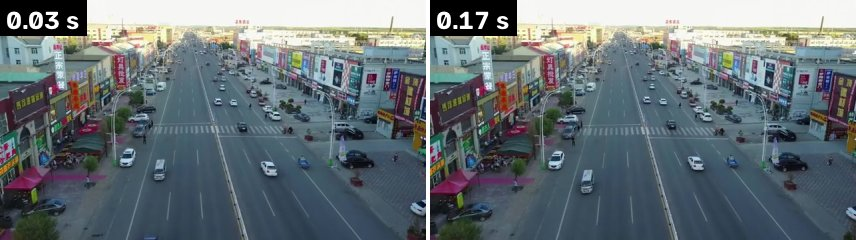
\includegraphics[height=20mm]{figures/failure_truncated.jpg} &
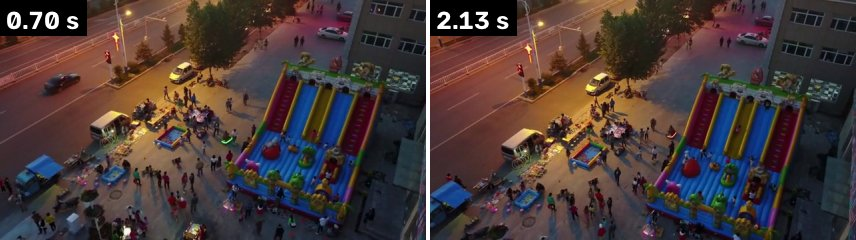
\includegraphics[height=20mm]{figures/failure_count.jpg} &
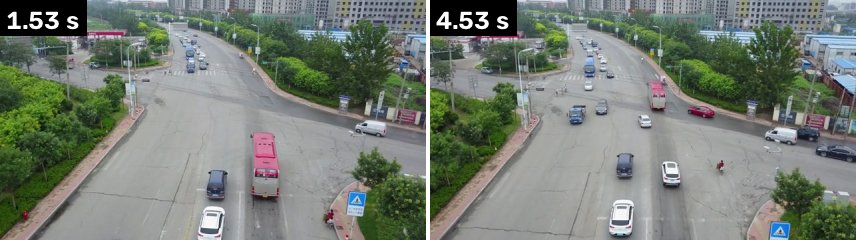
\includegraphics[height=20mm]{figures/failure_bus.jpg} \\[1pt]
\parbox[t]{0.32\textwidth}{\textbf{(a) TU\_Temporal}, 0.23\,s clip. How long is the white van
visible? Correct: \emph{0.0--4.0\,s}. Predicted: \emph{0.0--1.5\,s}.} &
\parbox[t]{0.32\textwidth}{\textbf{(b) FP\_ObjectLand.} How many parked vehicles are visible?
Correct: \emph{5--6}. Predicted: \emph{3--4}.} &
\parbox[t]{0.32\textwidth}{\textbf{(c) FP\_ObjectLand.} Where is the red bus as it moves through
the intersection? Correct: \emph{centre of the frame, toward the top}. Predicted: \emph{right side of
the road, moving away}.} \\
\end{tabular}}
\caption{Three failures of the fine-tuned model on dev: (a) a question that cannot be answered
because the clip is cut short, (b) counting too few small objects at dusk, (c) placing an object
in the wrong spot even though its motion is right. Labels give true times.}
\label{fig:errors}
\end{figure*}


\subsection{How good is the motion measurement on its own?}
Separately from any video model, we checked the motion probe against the
correct answers. We used the 862 training and validation camera-motion
questions whose answer is one of six classes: forward, backward, pan left,
pan right, rotating or stationary. From the probe's summary numbers alone,
we picked a class for each clip (Table~\ref{tab:confusion}).

The probe picks the correct class 73.0\% of the time. Always saying the
most common class (``forward'') would give 57.0\%. When we choose the
option that matches the probe's class, it answers 66.5\% of these questions
correctly (chance is 25\%). Forward flight is recognized in 454 of 491
cases.

Pans are the weak spot. In 60 of 111 ``panning right'' clips, the forward
part of the motion is larger in the clip summary, so the probe says
``forward''. We tried twice to fix this, both times with a pre-registered
plan, and both attempts failed or were inconclusive. Features that describe
the path separate the classes on average (the ratio of sideways to vertical
movement is 0.49 for pans vs.\ 0.14 for forward flight), but the two groups
overlap too much. Looking at the videos showed a deeper problem: on tilted
views, turning the camera (yaw) changes the perspective of the scene. Our
four-number model cannot represent that, so it reports a mix of pan and
rotation.

\begin{table}[t]
\centering
\caption{Motion probe alone vs.\ correct camera-motion answers (862
train+val questions; rows: correct class, columns: probe).}
\label{tab:confusion}
\footnotesize
\setlength{\tabcolsep}{4pt}
\begin{tabular}{@{}lrrrrrr@{}}
\toprule
 & back. & forw. & pan L & pan R & rot. & still \\
\midrule
backward ($n{=}23$) & \textbf{13} & 5 & 1 & 0 & 0 & 4 \\
forward ($n{=}491$) & 4 & \textbf{454} & 6 & 10 & 7 & 10 \\
pan left ($n{=}40$) & 4 & 15 & \textbf{9} & 2 & 4 & 6 \\
pan right ($n{=}111$) & 7 & 60 & 4 & \textbf{25} & 6 & 9 \\
rotating ($n{=}23$) & 1 & 5 & 2 & 1 & \textbf{13} & 1 \\
stationary ($n{=}174$) & 11 & 39 & 1 & 3 & 5 & \textbf{115} \\
\bottomrule
\end{tabular}
\end{table}
